% SynthAug-Bench paper.
% Journal-neutral draft: plain article class, one file per section in sections/.
% Moving to the chosen journal's template means swapping the class, the front matter and the
% bibliography style; the section files stay as they are.
% Tables and figures are read from the report (reports/Latex_report/), so each exists once.
% Compile from this folder: pdflatex main, bibtex main, pdflatex main, pdflatex main.

\documentclass[11pt]{article}
\usepackage[utf8]{inputenc}
\usepackage[T1]{fontenc}
\usepackage[margin=1in]{geometry}
\usepackage{amsmath,amssymb}
\usepackage{graphicx}
\usepackage{booktabs}
\usepackage{float}
\usepackage{xcolor}
\usepackage[colorlinks=true,linkcolor=blue,citecolor=blue,urlcolor=blue]{hyperref}

\graphicspath{{../../reports/Latex_report/fig/}{Fig/}}
\newcommand{\tabledir}{../../reports/Latex_report/tables}

% Inputs a generated table when it exists, otherwise prints a visible placeholder, so the draft
% compiles before every result is on main.
\newcommand{\resulttable}[1]{%
  \IfFileExists{\tabledir/#1.tex}{\input{\tabledir/#1.tex}}{%
    \begin{center}\fbox{\parbox{0.9\linewidth}{\centering\small\textcolor{red}{%
      Table pending: \texttt{\detokenize{#1}.tex}}}}\end{center}}}

% Marks text still to be written; remove every \todo before submission.
\newcommand{\todo}[1]{\textcolor{red}{[TODO: #1]}}

\title{SynthAug-Bench: When Does Synthetic Data Augmentation Help Image Classification?}
% TODO: final title once the main claim is fixed (candidate: the initialization sign flip).
\author{%
  Mayur Patil \and Manoj Kodihalli Venkatesh\\
  Data Science Program, The George Washington University
  % TODO: decide author order, the supervisor's role (co-author or acknowledgment) and emails.
}
\date{}

\begin{document}
\maketitle

\begin{abstract}
% Write last, once Results are final. Five sentences:
% (1) what this study shows, (2) why the question is hard and matters, (3) how it is tested,
% (4) the evidence, (5) the most important number.
% Every claim here must match a result in Section~\ref{sec:results}, on the test set.
% Candidate claims (each needs its test-set number before it goes in):
%   - Synthetic images beat RandAugment for ImageNet-pretrained classifiers at small budgets but lose
%     to it from random initialization (ResNet-50, ViT-B/16, ConvNeXt-T; 5 seeds; validation and test).
%   - Generator-quality measures (FID, precision, recall) rank the generated sets opposite to their
%     usefulness.
%   - A class-conditional GAN trained on the 5,000 real images shows the same sign flip.
\todo{abstract, five sentences, written last}
\end{abstract}

\section{Introduction}
\label{sec:intro}

% Paragraph plan (one message each):
%   1. Problem: generators can produce unlimited labelled images; when does adding them help a
%      classifier trained on scarce real data?
%   2. What is already known (synthetic data helps few-shot; FID predicts downstream use poorly) and
%      what is open (which set helps, and whether the answer depends on initialization).
%   3. This study: a controlled benchmark, paired seeds, matched step budgets, conventional
%      augmentation as the control.
%   4. Findings, then 2-4 contribution bullets of one or two lines each.
\todo{opening paragraphs 1-3}

% Moved from the report's Introduction. Its numbers are validation scores; replace them with the
% test-set numbers once the Results section is final.
\paragraph{Contribution.}
That synthetic images help when real data is scarce is expected: with 5 images per class, Stable Diffusion
class-prompt images raise ImageNet-pretrained ResNet-50 by 11.4 and ViT-B/16 by 14.5 points, in line with
earlier work on synthetic training data~\cite{he2023synthetic}. This study asks two questions that such
gains leave open. First, \emph{which property of a generated set predicts whether it will help?}
Generator-quality measures such as FID are known to predict poorly how well a classifier trained on
generated images performs~\cite{ravuri2019classification}, also for diffusion-based
augmentation~\cite{li2026diffusion}. We test this in the scarce-data setting, with the real images always
in the training set and conventional augmentation as a control. In our benchmark the two disagree:
among our three generated sets, the ones closest to the real training images help least. LoRA-adapted pools
are closer to the real data than class-prompt pools (lower FID and higher recall), and SD img2img edits of
the real images closer still, yet with pretrained classifiers the class-prompt set gives the largest gain at
every budget, and the img2img set a smaller gain than the LoRA set in 5 of 8 cells. No set-level measure we test, FID, precision or
recall, predicts which set will help, and in a first per-class analysis no precision, recall or diversity
measure predicts which classes gain. Second, \emph{why does the effect reverse with initialization?} The same images that help pretrained
classifiers lose to RandAugment for randomly initialized ones at most budgets. A recent systematic study of
diffusion-based augmentation~\cite{li2026diffusion} starts from ImageNet weights for some datasets and trains
from scratch on others, so it cannot separate the two, and it has no RandAugment control; our design pairs
both initializations on the same data, budgets and generated images. We test candidate explanations for
this sign flip (diversity of the generated images, their distance from the real data, and how well a
classifier trained on real images recognises them) and report which quality measures, if any, predict the
downstream gain. The aim is a practical rule for when to add generated images, and a warning about the
measures commonly used to choose them.

% TODO: add the GAN set (fourth generated set) and the Stage 2 checks (ConvNeXt-T, 2:1 and 5:1,
% Mixup/CutMix, stronger augmentation policies) to the paragraph above once their results are in.

\paragraph{Contributions.}
\todo{2-4 bullets, one or two lines each, each pointing to the section with its evidence}

\section{Related Work}
\label{sec:related}

% Moved from the report. Organized by method family; each subsection ends with how this study
% differs. Trim to about one page for the journal.

\subsection{Diffusion models and their adaptation}
A prominent line of research focuses on diffusion models and how to adapt them to new concepts. Ho et al.~\cite{ho2020denoising} introduced models that learn to undo noise step by step, allowing them to create images from pure noise. Rombach et al.~\cite{rombach2022high} made this cheaper by operating in a compressed latent space and adding text control via cross-attention, which forms the basis of Stable Diffusion. Because pretrained models only know what they saw during training, Gal et al.~\cite{gal2023image} proposed textual inversion to teach a frozen model one new ``word'' for a concept using a few images. Ruiz et al.~\cite{ruiz2023dreambooth} developed DreamBooth, which fine-tunes the entire model on a few images using a rare token and an extra loss so it does not forget original classes. Hu et al.~\cite{hu2022lora} introduced LoRA to train small low-rank matrices while freezing the main weights, offering a cheap adaptation method originally for language models but now common for diffusion. In contrast, this study combines LoRA with a DreamBooth-style token, training one specific adapter per data budget using only that budget's real images.

\subsection{Diffusion-based augmentation for classification}
A related approach uses diffusion models to edit existing real images for data augmentation. Trabucco et al.~\cite{trabucco2024effective} use image-to-image translation combined with a learned textual-inversion token for each class. They found that changing the background or pose while keeping the main object helps few-shot learning, even for plants the model never saw during training. Dunlap et al.~\cite{dunlap2023diversify} take this further by captioning real images and using a language model to suggest new domains, like different weather conditions. They edit the images to fit these new domains and filter out poor results, which beats normal augmentation on fine-grained data. In contrast, this study generates entirely new images from scratch instead of editing existing ones, and measures exactly when this helps across increasing data budgets from five examples up to the full set.
% TODO: this study now also has an img2img set (Section~\ref{sec:method}); reword "instead of editing".

\subsection{Synthetic images as training data}
Another line of work trains classifiers on images generated from class names or captions. He et al.~\cite{he2023synthetic} generate images with GLIDE using diverse prompts and filter them with CLIP, finding that synthetic data helps few-shot learning, though this gain shrinks as real data grows. Sariyildiz et al.~\cite{sariyildiz2023fake} train models solely on ``ImageNet clones'' made with Stable Diffusion, showing that prompt variety and lower guidance scale help these models transfer well to other datasets. Azizi et al.~\cite{azizi2023synthetic} fine-tune Imagen on all of ImageNet and show that adding the resulting synthetic images back into the real dataset improves accuracy. Lastly, Tian et al.~\cite{tian2023stablerep} learn representations by treating Stable Diffusion images with the same caption as positive pairs, achieving results comparable to training on real images. In contrast, this study adds synthetic images to scarce real data at a strict one-to-one ratio, restricts the diffusion adapter to only see its specific data budget, and compares the impact on both pretrained and from-scratch classifiers.
% TODO: the ratio is no longer only 1:1 (2:1 and 5:1 in Section~\ref{sec:results}); reword.

\subsection{Conventional augmentation and generators trained from scratch}
Beyond diffusion, other research relies on conventional data augmentation and generative models trained entirely from scratch. Cubuk et al.~\cite{cubuk2020randaugment} introduced RandAugment, which applies random standard transforms at one shared strength. It avoids an expensive policy search and is the conventional-augmentation baseline in this study. Karras et al.~\cite{karras2020training} developed StyleGAN2-ADA to train a GAN on just a few thousand images by augmenting what the discriminator sees, which prevents overfitting. GANs trained this way know only their training set, whereas Stable Diffusion carries knowledge from billions of outside images.
% TODO: the report said GANs were planned for later; this study now trains a class-conditional
% StyleGAN2-ADA on the 5,000 budget-50 images (Section~\ref{sec:method}). Say what it adds.
% TODO: add the other conventional controls used in the results, each with a verified reference
% (fetch every BibTeX field; do not write any from memory): AutoAugment, TrivialAugment, AugMix,
% Mixup, CutMix.

\subsection{Measuring generated-image quality}
A separate focus is measuring the quality of generated images. Heusel et al.~\cite{heusel2017gans} created the Fréchet Inception Distance (FID), which measures the distance between real and fake images using Inception features, where a lower score means higher similarity. Kynkäänniemi et al.~\cite{kynkaanniemi2019improved} improved on this by using k-nearest-neighbor regions to separate an image's realism (precision) from its variety (recall). Parmar et al.~\cite{parmar2022aliased} introduced Clean-FID to fix how FID scores inconsistently change with image resizing and compression. This study uses Clean-FID features, compares sets of equal size and reports a real-versus-real floor, so it can ask whether better FID leads to better accuracy.

\subsection{Beyond classification}
Recent work has also expanded generative data augmentation beyond simple image classification tasks. For example, Fang et al.~\cite{fang2024data} use controllable diffusion models to generate new objects directly inside bounding boxes. This creates labeled synthetic data for training object detection systems. Similarly, Xiao et al.~\cite{xiao2023multimodal} generate diverse images from existing captions to produce more training data for image captioning models. While both approaches help in low-data settings, this study currently focuses strictly on classification, leaving detection and captioning on datasets like COCO for later stages.
% TODO: keep as one sentence in the scope paragraph, or drop, depending on the journal's length.

\subsection{How this study differs}
In summary, this study differs from prior work through a highly controlled experimental design. It evaluates performance using the exact same protocol across five specific data budgets. The tests span both CNN and Transformer architectures, comparing classifiers trained from scratch against pretrained ones. This study specifically contrasts plain Stable Diffusion with per-budget LoRA adapters, ensuring training steps are matched so any accuracy gain is not simply from training longer. Furthermore, generated images are reduced to 32×32, the size of the real images, and this study compares the synthetic data with RandAugment and with the two combined. Finally, this study uses paired seeds to provide an explicit per-seed verdict on exactly when generative augmentation succeeds.

\section{Method}
\label{sec:method}

% Enough detail to reimplement; hyperparameters are in Section~\ref{sec:setup}.
% Use one term per concept throughout: real-only, data budget, generated images, generated set.

\subsection{Data and budgets}
% Moved from the report's protocol paragraph.
The study uses CIFAR-100~\cite{krizhevsky2009learning}. The split is fixed by a manifest with seed 42: 50 images per class (5,000 in total) are held out from the training pool for validation, and the 5, 10, 20 and 50 images-per-class budgets are nested subsets of the remaining 45,000 images, which form the full budget. The official 10,000-image test set is scored once per run, after the training and selection protocol was fixed.

\subsection{Classifiers}
% Moved from the report.
ResNet-50~\cite{he2016deep} and ViT-B/16~\cite{dosovitskiy2021image} are trained with all layers updated, either from ImageNet weights (torchvision \texttt{IMAGENET1K\_V2} and \texttt{IMAGENET1K\_V1}) or from random initialization. Images stay at $32\times32$ until they are upsampled to $224\times224$ on the GPU and normalized with the ImageNet statistics.
% TODO: ConvNeXt-T (Stage 2 check of the sign flip), with a verified reference.

\subsection{Training conditions}
% Moved from the report.
Each condition is defined as one change to the real-only control. \textit{Real-only} trains on the real images of the budget without augmentation. \textit{RandAugment}~\cite{cubuk2020randaugment} applies two RandAugment operations at magnitude 9 to every training image. \textit{Pretrained Stable Diffusion} adds generated images to the real-only training set, one generated image per real image (synthetic:real 1:1): for a budget of $k$ images per class, the first $k$ generated images of each class are added, so the generated sets are nested across budgets in the same way as the real ones. \textit{Pretrained Stable Diffusion with RandAugment} uses the same pool and applies RandAugment to every image, so that a gain from generated images can be separated from the gain of augmentation in general. \textit{LoRA-adapted Stable Diffusion} replaces the pool with images from an adapter fitted only on the real images of the same budget, so each budget has its own generated set.

Generated images are resized to $32\times32$ before training and then follow exactly the same preprocessing as the real images, so a classifier cannot separate the two by resolution or sharpness. Batches sample the combined pool uniformly, so about half of each batch is generated. Because the step budget stays the same as for real-only training, each image is seen about half as often as in the real-only run. Every run records a fingerprint of the generated pool, the synthetic:real ratio and the number of generated images it used.

% TODO: one sentence each for the other conditions in the results: SD-only (generated images
% alone), 2:1 and 5:1 ratios, Mixup and CutMix, TrivialAugment, AutoAugment and AugMix alone and
% combined with SD, and the GAN set below.

\subsection{Generated sets}
\label{sec:generated-sets}
\textbf{Class prompts.} \todo{Stable Diffusion 1.5, 25 steps, guidance 7.5, the eight prompt templates and the negative prompt; 450 images per class at $512\times512$, reduced to $32\times32$.}

\textbf{LoRA.} \todo{rank 8 on the U-Net attention projections, one adapter per budget fitted on that budget's real images only, with an identifier token.}

% Moved from the report.
\textbf{Image-to-image edits.} A third set, \textit{SD img2img}, edits the budget's own real images in the style of DA-Fusion~\cite{trabucco2024effective}: the same Stable Diffusion model, with the class prompts, changes each upsampled real image at strength 0.5, which keeps its layout and colours and adds detail. A run with $k$ images per class adds the edits of exactly its $k$ real images, so no other real image enters; this set covers 5 to 50 images per class.

\textbf{Class-conditional GAN.} A class-conditional StyleGAN2-ADA~\cite{karras2020training} is trained from random initialization on the 5,000 real images of the 50-images-per-class budget only, in the CIFAR configuration (batch 64, R1 weight 0.01, adaptive augmentation target 0.6). It is trained until the discriminator has seen 20 million real images, and the snapshot with the lowest FID against the same 5,000 images is kept (after 8 million images, FID 25.9 with 5,000 generated images). The set has 450 images per class, sampled without truncation, and is used only at the budget it was trained on.
% TODO: one sentence on the nearest-neighbour check (no copied training images) and a sample figure.

\subsection{Comparison and uncertainty}
% Moved from the report.
We compare conditions by the paired change for each training seed: the treatment score minus the control score of the same seed, in percentage points. A change counts as a gain or a loss only when every seed agrees in sign; otherwise it is reported as inconclusive.
% TODO: tables now use five seeds (0-4) in every reported cell; update this sentence and add the
% seed t-interval and the image bootstrap (moved to the appendix with their tables).

\begin{figure}[htbp]
	\centering
	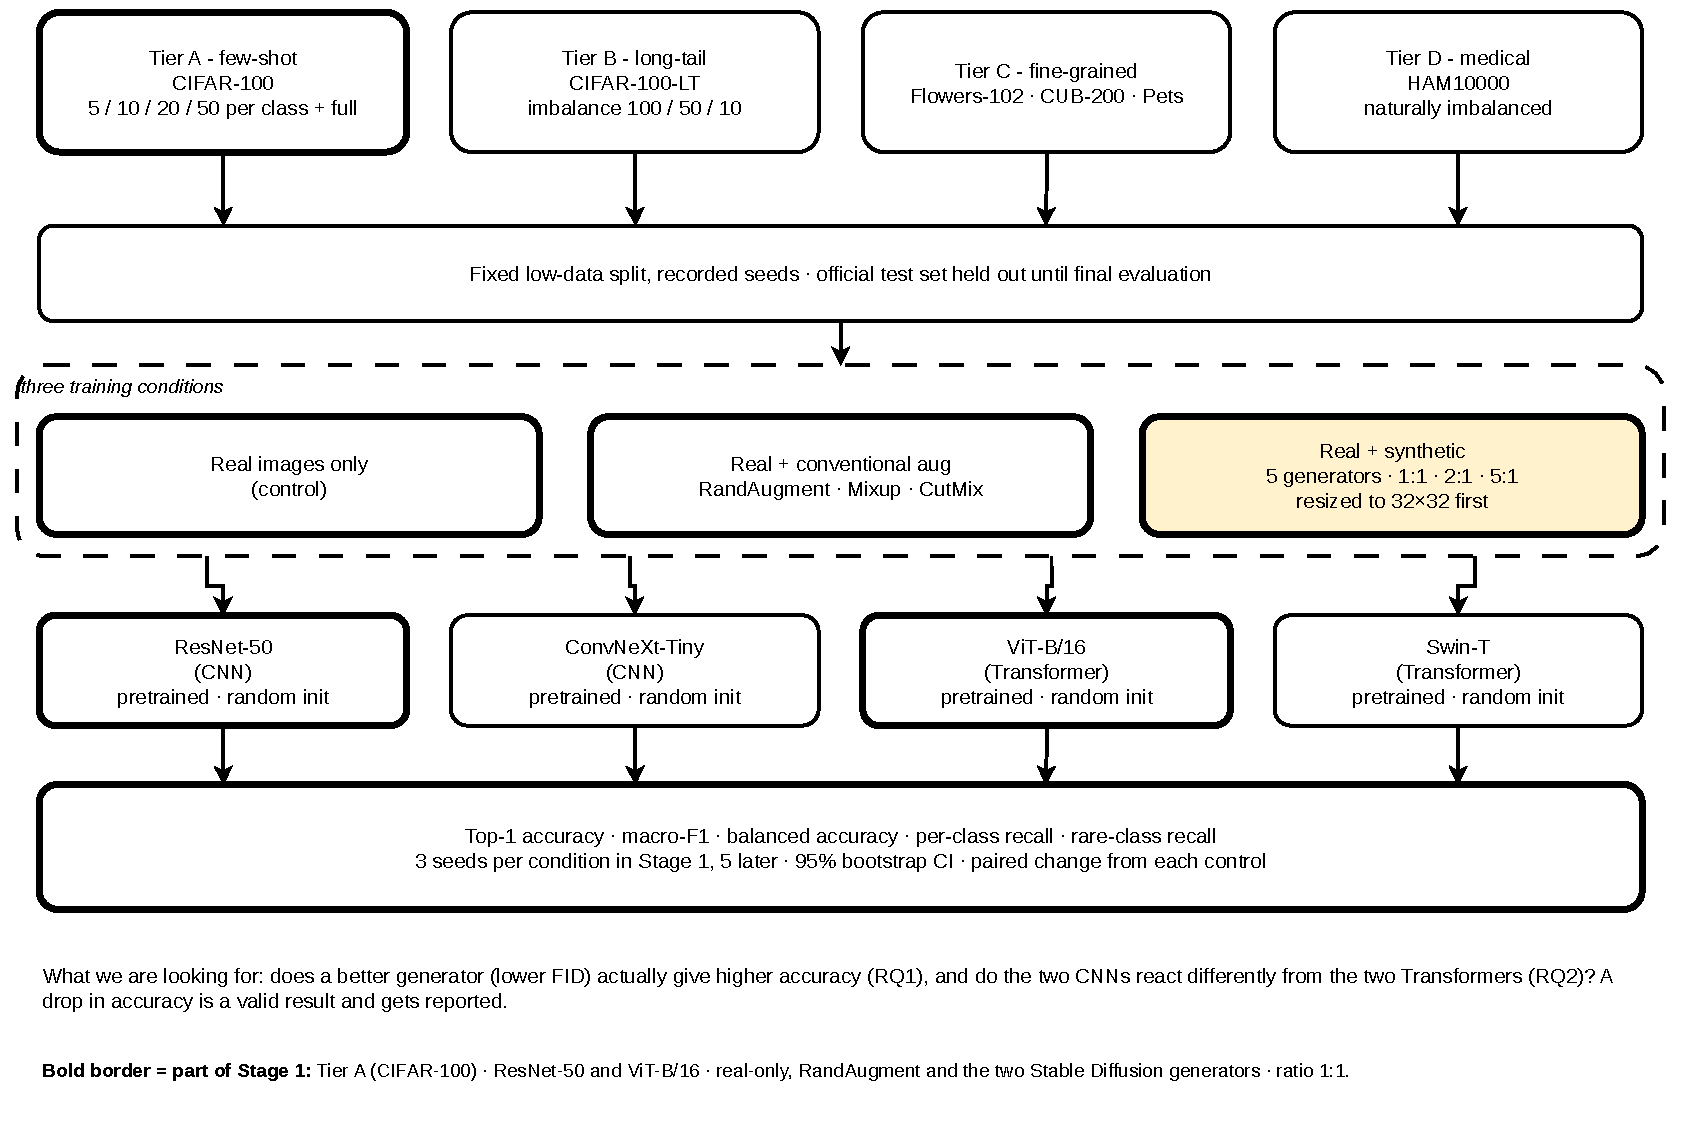
\includegraphics[width=\textwidth]{pipeline-2-classification.pdf}
	\caption{Classification study design. Each data tier is split once with recorded seeds, and the official
	test set is held out until the final evaluation. Every classifier, pretrained and randomly initialized,
	is trained under three conditions: real images only, real images with conventional augmentation, and
	real images with generated images, which are resized to the dataset's resolution first. Boxes with a
	bold border are part of Stage 1. \todo{redraw for the paper: only the CIFAR-100 tier and the
	classifiers and conditions that were run, plus the GAN set; drop the ``Stage 1'' wording}}
	\label{fig:classification-design}
\end{figure}

\section{Experimental Setup}
\label{sec:setup}

% Moved from the report's protocol section. Keep every number that a reader needs to rerun a cell.

\paragraph{Hardware and software.}
All runs used NVIDIA A10G GPUs (24\,GB). The pilots and the real-only and RandAugment runs used Python 3.12.14, PyTorch 2.12.1 (CUDA 12.6), Torchvision 0.27.1 and NumPy 2.5.2, the versions pinned in the environment file. The synthetic-data runs with seeds 0 to 2 were trained on a second A10G instance with Python 3.13.14, PyTorch 2.13.0 (CUDA 13.0), Torchvision 0.28.0 and NumPy 2.4.4; their seed 3 and 4 runs used the pinned versions.
% TODO: add the Stage 2 note (seeds 0-2 in the newer environment, paired with pinned controls) and
% the GAN runs (pinned environment), then total runs and GPU hours.

\paragraph{Training recipe.}
Every run uses batch size 128, linear warmup over the first 5\% of steps followed by cosine decay to zero, label smoothing 0.1, gradient-norm clipping at 1.0 and bf16 mixed precision. The real-only condition applies no augmentation; RandAugment applies two operations at magnitude 9 to the $32\times32$ image.

\paragraph{Learning rates and step budgets.}
The learning rates and optimizer-step budgets were chosen in pilot runs with seed 100, on validation accuracy only (38 runs, 21.2 GPU hours). The pretrained arm uses AdamW with weight decay 0.05 and learning rate $3\times10^{-4}$ for ResNet-50 and $5\times10^{-5}$ for ViT-B/16, for 600, 800, 1,000, 1,500 and 6,000 steps at the five budgets. The random-initialization arm uses SGD with momentum 0.9, weight decay $5\times10^{-4}$ and learning rate 1.0 for ResNet-50, and AdamW with weight decay 0.05 and learning rate $3\times10^{-4}$ for ViT-B/16, for 2,000, 3,000, 4,000, 8,000 and 50,000 steps. Within an arm, every condition of a given budget uses the same recipe and step budget.
% TODO: ConvNeXt-T rates from its pilot (pretrained 1e-4, scratch 3e-3).

\paragraph{Checkpoint selection and seeds.}
Each run is validated 20 times at equal step intervals and keeps the checkpoint with the highest validation accuracy, breaking ties by the lower validation loss and then the earlier step. The batch order and per-sample augmentation are fixed functions of the seed and the step.
% TODO: state the final seed count per cell (0-4) and the number of runs per study.

\section{Results}
\label{sec:results}

% Test-set results in the main text, validation results in the appendix. Before each experiment,
% state the claim it tests. Every number is a paired change over seeds 0-4 (mean, sample SD, verdict).
% Tables are generated by src/component/analyze_results.py and stage2_results.py (--split test);
% the test tables appear here once they are on main.

\subsection{Synthetic images with pretrained classifiers}
\label{sec:results-pretrained}
\todo{claim and numbers: class-prompt images vs real-only and vs RandAugment, pretrained, by budget (test)}

\resulttable{stage1_pretrained_test_accuracy_sd_prompt}
\resulttable{stage1_pretrained_test_accuracy_vs_randaugment}

\subsection{The sign flip with initialization}
\label{sec:results-flip}
\todo{claim and numbers: the same images lose to RandAugment from random initialization; ResNet-50,
ViT-B/16 and ConvNeXt-T, every seed (test)}

\resulttable{stage1_scratch_test_accuracy_vs_randaugment}
\resulttable{stage2_convnext_pretrained_test}
\resulttable{stage2_convnext_scratch_test}

\subsection{More generated images per real image}
\label{sec:results-ratio}
\todo{claim and numbers: 1:1, 2:1, 5:1; all 36 ratio-vs-real comparisons are gains on validation and
test; from scratch 5:1 beats RandAugment in 3 of 4 cells}

\resulttable{stage2_ratio_pretrained_test}
\resulttable{stage2_ratio_scratch_test}

\subsection{Stronger conventional augmentation}
\label{sec:results-augment}
\todo{claim and numbers: Mixup, CutMix, TrivialAugment, AutoAugment and AugMix alone and combined
with class-prompt images, from random initialization; augmentation seeds 1-4 are still running}

\resulttable{stage2_mixing_pretrained_test}
\resulttable{stage2_mixing_scratch_test}
% TODO: table for the policy and stacked conditions (runs/augment-scratch) once all seeds are in.

\subsection{A generator trained only on the real images}
\label{sec:results-gan}
\todo{table of the GAN set at 50 images per class, both initializations, test, 5 seeds}
% Test-set paired changes, GAN minus real-only, mean over seeds 0-4 (from runs/gan-*):
%   pretrained ResNet-50 -2.97, ViT-B/16 -3.50 (0/5 seeds positive);
%   scratch ResNet-50 +4.59, ViT-B/16 +3.89 (5/5 positive).
%   Scratch ViT-B/16: GAN minus SD class prompts +0.65 (5/5); scratch ResNet-50: -4.06 (0/5).
% Generate the table with a script before quoting these numbers in text.

\subsection{Does generator quality predict usefulness?}
\label{sec:pool-utility}
% Moved from the report (validation scores; check against the test scores before submission).
FID and Improved Precision \& Recall describe a generated set without training on it. To test whether they
predict which set helps more, we compare the generated sets of each budget: SD class prompts, the LoRA set
of that budget and the SD img2img edits of the budget's own real images (5 to 50 images per class; the full
set has the first two). Every pair of sets is compared within each budget, classifier and initialization
(52 comparisons). A comparison agrees when the set a measure rates better also gives the larger paired gain
over real-only, averaged over the seeds both sets share (seeds 0--2). Comparing within a budget is
necessary: both FID and the gain shrink as the budget grows, so across budgets any measure would appear to
predict the gain through the budget alone.

Two details of the measurement matter. First, the img2img edits and the LoRA adapter are made from the
budget's own real images, and a reference sample drawn from the whole training pool contains some of them
(6 of 500 reference images at 5 images per class, up to 557 of 5,000 at 50), which would flatter those sets.
From 5 to 50 images per class, all three sets are therefore scored against a reference that leaves the
budget's images out. This moves the img2img FID by at most 1.5 (94.1 to 95.5 at 5 images per class) and
changes no conclusion below. Second, the comparisons are not independent: a measure rates each pair of
sets once per budget, and the two classifiers and two initializations of that budget share the verdict.
Where a pair's verdict is the same at every budget, the measure agrees exactly where the favoured set wins,
so we test a measure only on the pairs whose verdict changes between budgets. FID minus the
real-versus-real floor is not a separate measure, since the sets of a budget share the floor.

Table~\ref{tab:pool-utility} and Figure~\ref{fig:pool-utility} give the result. The usefulness of the three
sets follows one order. The class-prompt set gives a larger gain than the LoRA set in 17 of 20 comparisons
(all 10 with pretrained classifiers, in 29 of 30 seed pairs) and than the img2img set in all 16, and the
LoRA set a larger gain than the img2img set in 13 of 16. FID and recall rank the sets in the opposite order
at every budget: img2img first, then LoRA, then class prompts. They pick the more useful set in only 6 of 52
comparisons, the few where the order of usefulness is reversed: the LoRA set ahead of the class-prompt set
in three cells from random initialization (ResNet-50 at 20 images per class, and both classifiers on the
full set, by 2.4 and 2.1 points), and the img2img set ahead of the LoRA set in three pretrained cells at 20
and 50 images per class. Because their verdict never changes, we give them no $p$-value, but the pattern is
plain: the sets that these measures rate closest to the real data help least.

Precision rates the class-prompt set above both others at every budget and so agrees in 42 of 52
comparisons, but that count mostly restates that the class-prompt set wins. The one pair whose precision
verdict changes between budgets is LoRA against img2img (LoRA ahead at 10 and 20 images per class, img2img
at 5 and 50, by 0.01 to 0.02), and there precision picks the more useful set in 9 of 16 comparisons, at
chance ($p = 0.80$). The third set thus answers the question that two sets left open: none of the three
measures predicts which generated set will help beyond the advantage of the class-prompt set.

The order of usefulness matches how far each set is from the budget's own real images. The class-prompt
images never see them, the LoRA adapter is fitted to them, and the img2img edits keep their layout and
colours. One explanation consistent with this order, which we have not tested directly, is that in the
scarce-data setting a generated set helps by adding what the few real images lack, while FID and recall
reward closeness to the real data and so rank the sets the wrong way round. The order also
holds from random initialization, where the class-prompt set is ahead of the img2img set in all 8
comparisons and by 3.4 and 5.7 points for ResNet-50 at 20 and 50 images per class.
% TODO: add the GAN set at 50 images per class (FID 25.9 vs its own training images; measure it
% with the same reference and floor as the other sets before comparing).

\resulttable{pool_utility_summary}

\begin{figure}[H]
\centering
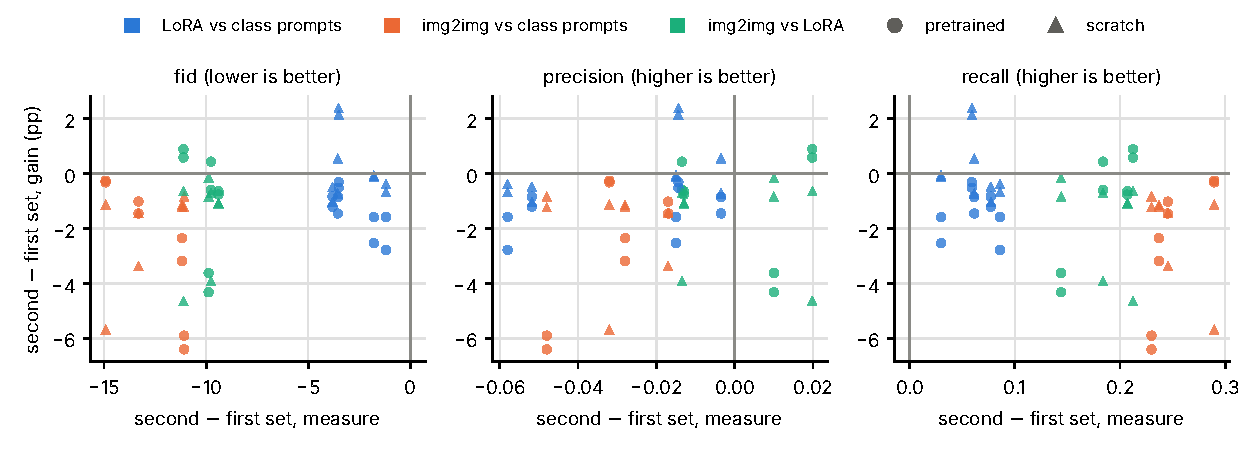
\includegraphics[width=\textwidth]{pool_utility_measure_vs_gain.pdf}
\caption{For each pair of generated sets (colour), the second set minus the first, in each quality
measure (x) and in the paired gain over real-only (y), one point per budget and classifier; circles:
pretrained, triangles: random initialization. A measure that predicts usefulness puts the points in the two
quadrants where its sign matches the gain's (for FID, lower is better, so the upper-left and lower-right
quadrants). The scores at 5 to 50 images per class use a reference without the budget's own images.}
\label{fig:pool-utility}
\end{figure}

\subsection{Why the effect flips with initialization}
\label{sec:sign-flip}
% Moved from the report (validation and training images only).
SD class-prompt images raise the accuracy of ImageNet-pretrained classifiers at every budget but lose to
RandAugment for randomly initialized ones at most budgets. We tested two explanations on validation and
training images only.

\paragraph{Diversity and per-class distance do not explain it.}
For each class we compared 50 generated with 50 real training images in Inception feature space:
Improved Precision and Recall within the class, the spread of the generated images relative to the real
ones, and the distance between the two class means. The generated images are realistic but narrow
(mean per-class precision 0.73, recall 0.26, spread 0.86 of the real class). None of these measures
predicts the per-class recall change of SD over real-only at 5 images per class, for either
initialization ($|\rho| \le 0.19$, no permutation $p$ below 0.05 over the 100 classes). Over all 60
correlations we computed, the only ones that survive a Holm correction concern the change
of scratch ResNet-50 over RandAugment (precision $\rho = +0.36$, Holm $p = 0.024$), and they come from
RandAugment's own per-class gain ($\rho = -0.40$, Holm $p = 0.006$), not from SD. With 100 classes a
correlation must exceed about 0.20 to reach $p < 0.05$, and only true correlations of about 0.28 or more
are detected with 80\% power, so weaker per-class effects may be missed.

\paragraph{A real-only classifier recognises the generated images less well from scratch.}
Table~\ref{tab:synthetic-accuracy} gives the accuracy of classifiers trained on real images only on
5{,}000 generated images (50 per class), next to their accuracy on the real validation images. Pretrained
classifiers recognise the generated images almost as well as real ones (93--97\% of their validation
accuracy on the full training set, 99\% at 5 images per class). Classifiers trained from scratch lose
about 9 points on them even with the full training set (79--83\%). The generated images are faithful to
their class, which answers how good the generation is, but they lie in a region that features learned
from CIFAR-100 alone cover less well. A pretrained backbone bridges this shift; a network trained from
scratch must learn both distributions from the same few images, and the generated images help it less
than RandAugment's perturbations of the real ones. Per class, the accuracy of the full-data real-only
classifiers on the generated images is weakly but consistently related to the gain of SD over real-only
($\rho = 0.15$--$0.29$ over the four classifiers, none significant after the Holm correction). For
pretrained classifiers this relation is specific to SD ($\rho = 0.06$--$0.08$ for RandAugment); from scratch
it is about as strong for RandAugment ($\rho = 0.16$--$0.19$), so there it partly reflects how easy a class
is. Because the per-class relations are weak, the shift appears to be a property of the generated set as a
whole rather than of particular classes.

\begin{table}[H]
\centering
\small
\caption{Accuracy (\%) of real-only classifiers (seed 0) on the real validation images and on 5{,}000 SD
class-prompt images (50 per class), and the second as a share of the first. At 5 images per class the
scratch classifiers are close to chance (1\%), so their ratios are noisy.}
\label{tab:synthetic-accuracy}
\begin{tabular}{llrrrr}
\toprule
Initialization & Model & Images/class & Real val. & Generated & Ratio \\
\midrule
Pretrained & ResNet-50 & full & 84.22 & 78.24 & 0.93 \\
Pretrained & ViT-B/16  & full & 88.62 & 85.84 & 0.97 \\
Scratch    & ResNet-50 & full & 54.44 & 45.14 & 0.83 \\
Scratch    & ViT-B/16  & full & 43.72 & 34.44 & 0.79 \\
\midrule
Pretrained & ResNet-50 & 5 & 35.66 & 35.46 & 0.99 \\
Pretrained & ViT-B/16  & 5 & 45.14 & 44.78 & 0.99 \\
Scratch    & ResNet-50 & 5 & 8.60  & 6.00  & 0.70 \\
Scratch    & ViT-B/16  & 5 & 7.74  & 6.72  & 0.87 \\
\bottomrule
\end{tabular}
\end{table}

These results come from one seed per classifier.
% TODO: the direct test is now done: SD-only (generated images alone, validated on real images) for
% both initializations; add its result here. The GAN set, which shares the classifiers' pixel
% statistics, is a second test of the distribution-shift explanation.

\section{Discussion}
\label{sec:discussion}

% One message per paragraph:
%   1. A practical rule: when to add generated images (pretrained backbone, small budget) and when a
%      conventional policy is the better use of the step budget (random initialization).
%   2. What the quality measures miss, and what to measure instead.
%   3. What the GAN set adds: a generator with no outside knowledge shows the same pattern, so the
%      flip is not specific to Stable Diffusion's pretraining data.
%   4. Where the explanations stop: what is tested and what is only consistent with the data.
\todo{discussion, four paragraphs as planned above}

\section{Limitations}
\label{sec:limitations}

% Moved from the report. State each weakness and why it does not undermine the main claims.

\textbf{One dataset at low resolution.} The study uses CIFAR-100 only, and its $32\times32$ images are upsampled to $224\times224$ for the classifiers. Results may differ for datasets with larger images or other domains.

\textbf{Seeds.} \todo{rewrite for five seeds (0-4) in every reported cell; the report's version described three.} With few training seeds, a gain or loss is declared only when all seeds agree, and the standard deviations are themselves uncertain. In the baselines, the standard deviation of the paired change reaches 4.7 points (ResNet-50 from random initialization, 50 images per class), so the study can resolve only effects larger than this spread; smaller effects are reported as inconclusive.

\textbf{Fixed step budgets.} The step budgets were chosen in pilots on the real-only condition and are equal across conditions, so the comparison holds the training compute fixed. Some runs reached their best validation score at the final step: in the pretrained arm 1 of 30 real-only and 8 of 30 RandAugment runs, and in the random-initialization arm 6 of 30 and 13 of 30. Because the cosine schedule ends at a learning rate of zero, the last steps are often the best, but augmented runs might also gain from longer training, so the RandAugment gains may be understated. In the synthetic-data conditions the same step budget is spread over twice as many images, so each real image is seen about half as often as in the real-only run; the exposures are recorded for every run.

\textbf{One fixed recipe from scratch.} \todo{absolute accuracy from random initialization is low (best at the full budget about 65\%) because every condition shares one recipe and step budget; say why this is the right control and what it costs.}

\textbf{Outside pretraining.} The ImageNet weights of the pretrained classifiers and the web-scale training data of Stable Diffusion are outside our control. The diffusion training data may contain images similar to, or taken from, CIFAR-100, so any benefit of generated images may partly reflect that exposure. The random-initialization arm removes the classifier's outside knowledge but not the generator's.
% TODO: the GAN set removes the generator's outside knowledge too; say so here.

\textbf{Two software environments.} The synthetic-data runs with seeds 0 to 2 were trained with newer Python, PyTorch, Torchvision and NumPy versions than the real-only and RandAugment runs they are paired with (Section~\ref{sec:setup}). For seeds 3 and 4, both sides of each pair used the same versions. The recipe, split and step budgets are identical, but a version change can shift accuracy slightly, so small paired changes between the two groups should be read with that in mind.
% TODO: if the baseline rerun in the newer environment is done, give the measured shift.

\section{Conclusion}
\label{sec:conclusion}

% A short answer to each research question, each tied to its result section; no new claims.
\todo{conclusion: one short answer per research question}


\bibliographystyle{IEEEtran}
\bibliography{references}

\appendix
\section{Validation results and uncertainty}
\label{app:validation}

% Validation tables moved from the report; the main text uses the test set.

\resulttable{stage1_pretrained_accuracy}
\resulttable{stage1_scratch_accuracy}
\resulttable{stage1_pretrained_accuracy_sd_prompt}
\resulttable{stage1_pretrained_accuracy_vs_randaugment}
\resulttable{stage1_scratch_accuracy_vs_randaugment}

\section{Seed intervals and image bootstrap}
\label{app:bootstrap}
% Moved from the report's error analysis (validation predictions; no retraining, test set unused).
\todo{move the report's uncertainty paragraph here, updated to five seeds}

\resulttable{stage1_pretrained_bootstrap}
\resulttable{stage1_scratch_bootstrap}

\section{Per-superclass changes}
\label{app:superclass}

\begin{figure}[H]
	\centering
	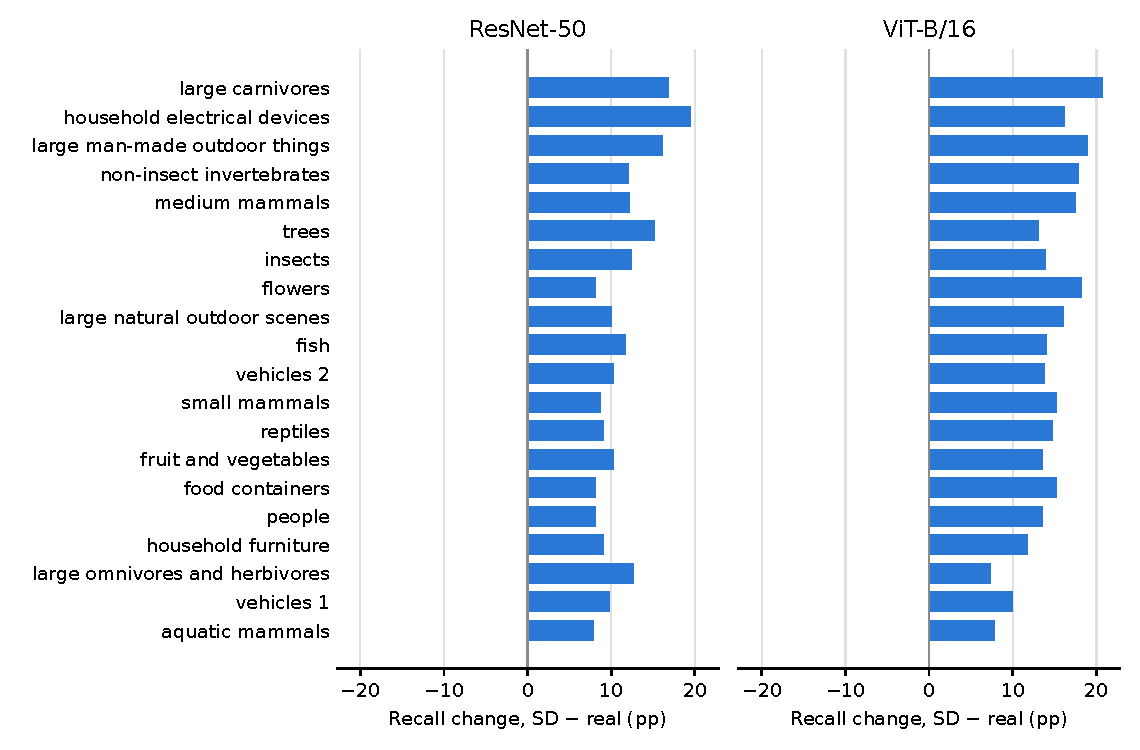
\includegraphics[width=0.85\textwidth]{stage1_pretrained_b5_sd_prompt_vs_real_only_superclasses.pdf}
	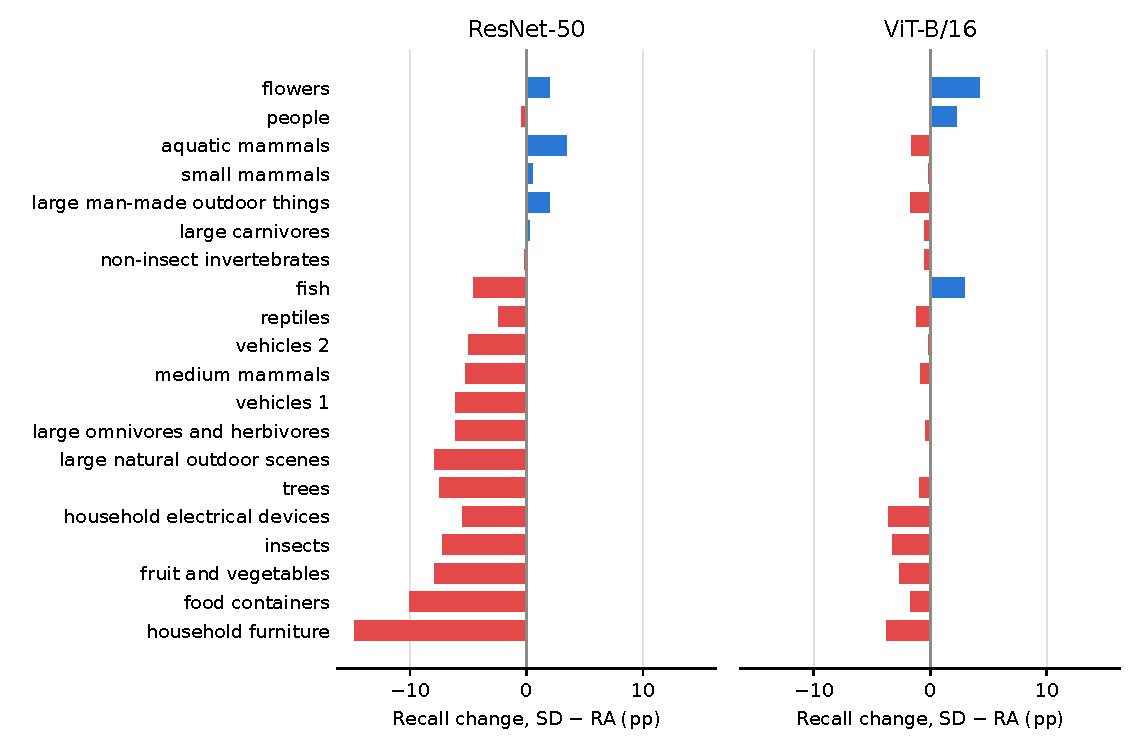
\includegraphics[width=0.85\textwidth]{stage1_scratch_b5_sd_prompt_vs_randaugment_superclasses.pdf}
	\caption{Recall change per CIFAR-100 superclass at 5 images per class, mean over seeds 0 to 4 (top) and 0 to 2 (bottom), in percentage points. Top: class-prompt images minus real-only, ImageNet-pretrained classifiers. Bottom: class-prompt images minus RandAugment, randomly initialized classifiers. Superclasses are sorted by the mean change over both models; blue bars are gains and red bars losses.}
	\label{fig:stage1-superclass}
\end{figure}

\section{Generated samples}
\label{app:samples}

\begin{figure}[H]
	\centering
	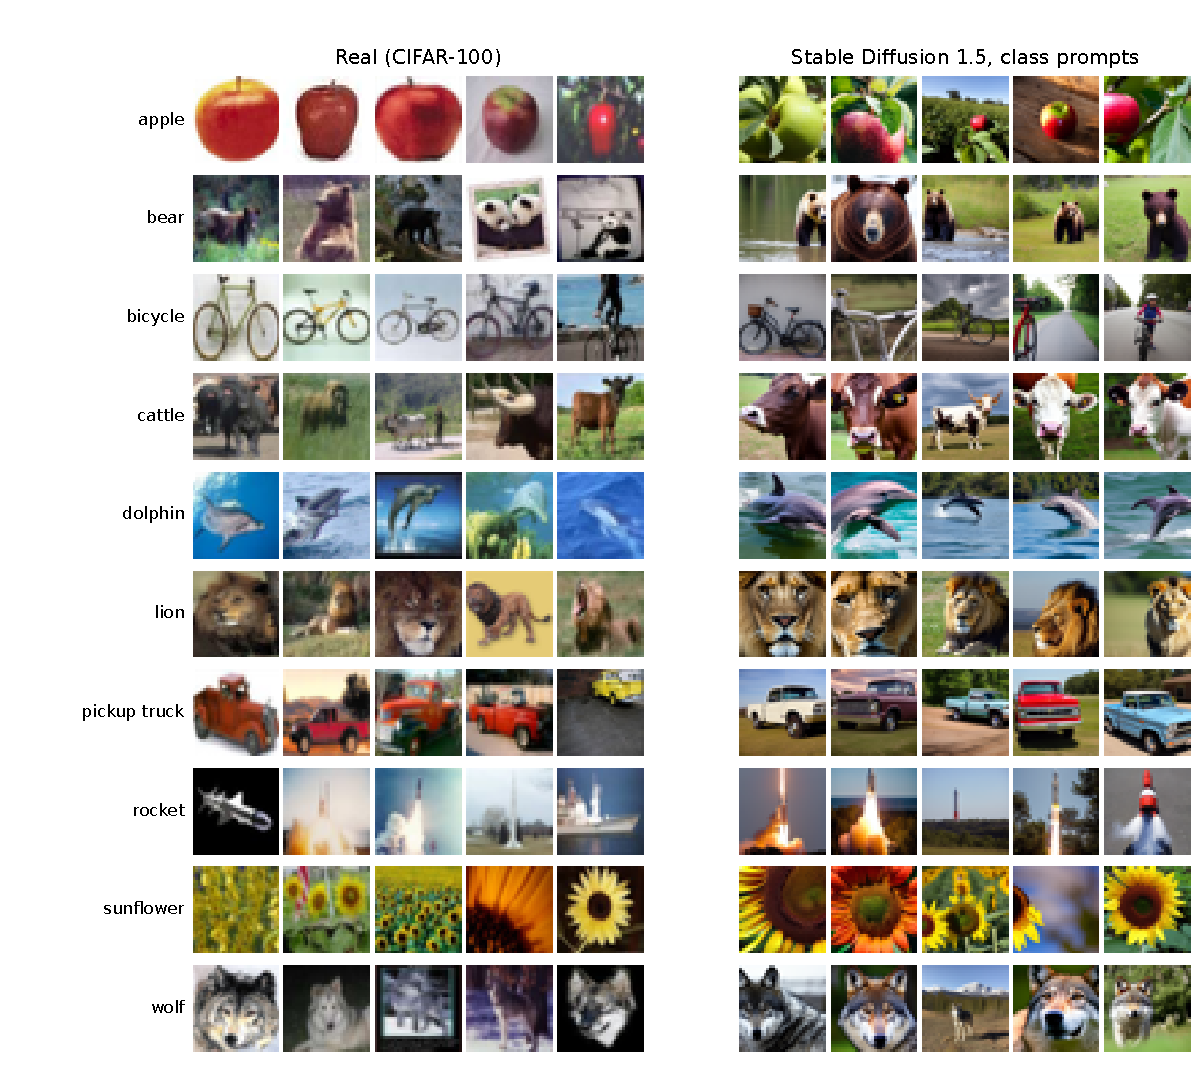
\includegraphics[width=0.8\textwidth]{sd15_prompt_samples.pdf}
	\caption{Samples of the class-prompt pool (pretrained Stable Diffusion 1.5, 32$\times$32 as used for training).}
	\label{fig:sd-samples}
\end{figure}
% TODO: LoRA, img2img and GAN samples side by side.


\end{document}
